%\documentclass{article}
\documentclass[twocolumn]{article}
\usepackage[utf8]{inputenc}
\usepackage{tikz}
\usetikzlibrary{positioning,fit,shapes,arrows.meta}

\author{ K\'evin Le Bon \and Alan Schmitt }

\title{MLExplain}

\begin{document}
\maketitle

\begin{abstract}
  MLExplain is a step-by-step interpreter for OCaml that enables the
  user to inspect both their program's state and the interpreter's state
  itself. This interpreter aims to provide the user with a better understanding
  of the semantics of OCaml.
\end{abstract}

\section{Introduction}

The semantics of a programming language can be very complex. When a language
has no specification, the semantics is then defined by the implementations of
the language, i.e., interpreters and compilers. However even when a
specification is available, it can be difficult to understand why the execution
of a specific program results to a certain output.

The goal of the \emph{JSExplain} project \cite{chargueraud:hal-01745792} is to
describe the execution of a JavaScript program by showing every step of an
interpreter whose behavior is very close to the specification of JavaScript. In
this paper, we show how we adapted JSExplain to OCaml.

Unlike JavaScript, OCaml has no official specification. However, OCaml code
execution is fairly simple because the number of language constructions is
small. We have written an interpreter for OCaml's typed abstract syntax tree
(AST). This AST is still close to the source code yet it provides additional
crucial information. For instance, it mentions resolved names, which is useful
for module and signatures inclusion and mandatory for interpreting features like
named parameters and optional parameters in functions. The semantic we give to
OCaml is higher level than the one described in \emph{ZINC} \cite{Leroy-ZINC}
virtual machine, i.e., an interpreter for bytecode after compilation.

\section{JSExplain}

\subsection{A Double Debugger}
\label{subsec:double-debugger}

We call a \emph{double debugger} an interpreter that is able to run step by step
and display the program's state and current location in source, as well as the
state and location in the source of the interpreter itself. JSExplain is a
double debugger for JavaScript. The aim of this tool is to help a user to better
understand JavaScript's semantics, by providing an interpreter that is very
close to the specification of JavaScript. JSExplain's interface highlights the
expression of the program currently evaluated as well as the instruction of the
interpreter that is executed.

\subsection{Architecture}

The core of JSExplain is a JavaScript interpreter written in a subset of OCaml.
This interpreter is compiled to a subset of JavaScript and instrumented to
generate a trace of its execution when run. This trace can then be navigated
using a web-based
tool.\footnote{https://jscert.github.io/jsexplain/branch/master/driver.html}

The subset of OCaml we support for writing the interpreter is purely functional
with variables, constants, sequence, conditional, let-binding, function
definition, function application (with support for prefix and infix functions),
data constructors, records (including record projections, and the
``record-with'' construct to build a copy of a record with a number of fields
updated), tuples (i.e., anonymous records), and simple pattern matching (only
with non-nested patterns, restricted to data constructors, constants, variables,
and wildcards). For convenience, let-bindings and functions may bind simple
patterns (as opposed to only variables). We also support \texttt{ppx} extensions
for monadic programming, to simplify the handling of errors.

The target language of our compiler is a purely functional subset of JavaScript
where there is never any type conversion, where objects are used as records (no
use of their \texttt{prototype} field), and where tuples are encoded into
arrays.

We instrument the compilation to JavaScript by adding code that logs events,
namely entering a function, creating a scope, assigning a variable, and exiting
a function. Each event captures the state, the stack, and the values of all
local variables in scope of the interpreter code at the point where the event
gets triggered. Code that is traced is compiled with this instrumentation,
whereas code that is not traced, for instance supporting libraries, is directly
compiled to JavaScript.

When using the tool, the source JavaScript program is parsed and run through the
instrumented interpreter, thus generating a trace. We can then navigate this
trace to see the state of the interpreter as well as the state of the
interpreted program. Recovering the information about the interpreted code is
not completely straightforward. For example, to recover the fragment of code to
highlight, we find in the trace the closest previous event that contains a call
to function with an argument named \texttt{\_term\_}. This argument corresponds
to the AST of a subexpression, and this AST is decorated (by the parser) with
locations. Note that, for efficiency reasons, we associate to each event from
the trace its corresponding \texttt{\_term\_} argument during a single pass,
performed immediately after the trace is produced.

Similarly, we are able to recover the state and environment associated with the
event. The state of the interpreted program consists of four fields: the
strictness flag, the value of the \texttt{this} keyword, the lexical
environment, and the variable environment. We implemented a custom display for
these elements, and also for values of the languages, in particular for objects:
one may click on an object to reveal its contents and recursively explore it.

Finally, a web interface is presented to the user, to navigate in the trace.
This navigation can be forward and backward, and at all times the source code
and interpreter code are highlighted, and their states are displayed. We also
provide a way to specify breakpoints, using arbitrary JavaScript expressions,
that reference both the interpreter and interpreted programs. One may thus reach
a point where some interpreter line is being evaluated with some source value
satisfying a predicate, or vice-versa.

\section{MLExplain}

At first glance, JSExplain seems tightly linked to JavaScript. However, the
architecture of the project actually lets us completely replace the interpreter
with one for a different language. Our main task was to create a new OCaml
interpreter that could be integrated into the rest of the application. Then, we
noticed that the web application itself needed some changes -- for instance to
pretty print values.

% Plus de blabla

\subsection{Two compilers}

\begin{figure*}[t]
  \centering
  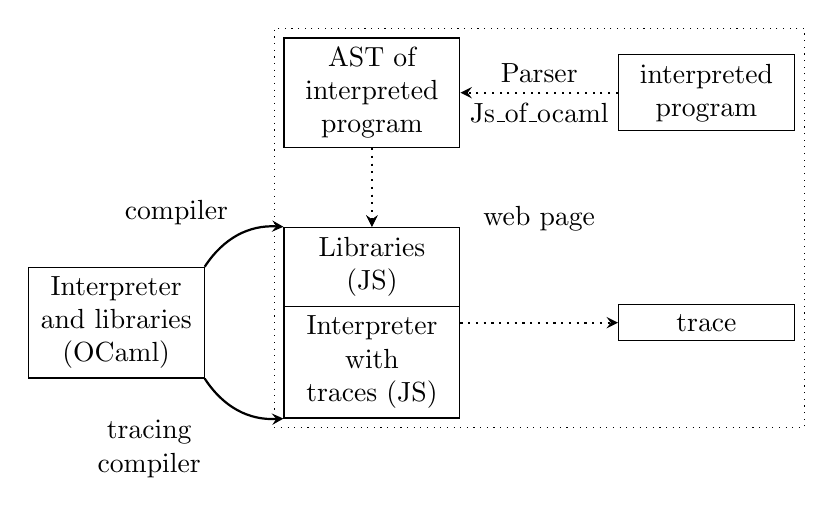
\begin{tikzpicture}[nodes = {align = center}]
    \node (focaml) [draw, text width=2cm] {Interpreter and libraries (OCaml)};

    \node (fjs) [draw, right = 1cm of focaml, text width=2cm, rectangle split,
    rectangle split parts=2, text centered] {Libraries (JS) \nodepart{second}
      Interpreter with traces (JS)};

    \node (ast) [draw, above = of fjs, text width=2cm] {AST of interpreted
      program};

    \node (source) [draw, right = 2cm of ast, text width=2cm, text centered]
    {interpreted program};

    \node [draw, dotted, fit=(fjs) (ast) (source)] {web page};

    \node (trace) [draw, right = 2cm of fjs, text width=2cm, text centered]
    {trace};

    \path[->,thick,>=stealth] (focaml.north
    east) edge[bend left] node[above left] {compiler} (fjs.north west) ;

    \path[->,thick,>=stealth] (focaml.south east) edge[bend right] node[below
    left] {\parbox{2cm}{\centering tracing compiler}} (fjs.south west);

    \path[->,thick,dotted,>=stealth] (source) edge node [above] {Parser} node
    [below] {Js\_of\_ocaml} (ast);

    \path[->,thick,dotted,>=stealth] (ast) edge (fjs);

    \path[->,thick,dotted,>=stealth] (ast) edge (fjs);

    \path[->,thick,dotted,>=stealth] (fjs) edge (trace);
  \end{tikzpicture}
  
  \caption{Architecture of MLExplain}
  \label{fig:archi}
\end{figure*}

To interpret OCaml code, we need to parse and type it. However, our compiler
does not allow us to use the standard library nor an external one. Fortunately,
JSExplain itself did not trace both parsing and typing processes. That is why
we have been able to separate totally the frontend from the interpreter itself
and use another compiler to compile it. The figure \ref{fig:archi} describes
the architecture of the whole application.

The frontend is compiled with \emph{js\_of\_ocaml}
\cite{DBLP:journals/spe/VouillonB14}, the compiler of the project
\emph{Ocsigen} \cite{balat:hal-00691710}. The largest part of the frontend is a
module that serializes the \emph{Typedtree} -- the typed AST of OCaml -- into a
JavaScript object compatible with the backend interpreter's own representation
of the AST. We use the \texttt{compiler-libs} library to do the actual parsing
and typing. We ensure that the typed AST we get is the same as the official
OCaml compiler AST since we use the exact same frontend.

% TODO: Alan, si tu as une idée pour raccourcir ou découper cette phrase
The main reason why both AST representations are not compatible and require an
explicit hand-made serialization into JavaScript is how the compilers compile
OCaml type constructors. Our compiler creates a JavaScript object from the type
and treats constructors as methods building themselves the value. This value is
a simple JavaScript object. \emph{js\_of\_ocaml}, on the other hand, uses its
own internal representation of OCaml value that we cannot use directly.

\subsection{Solutions to compiler limitations}

As stated before, the backend of our interpreter had to be written in
\texttt{fOCaml} to be integrated into the web interface. This limitation forced
to write non-idiomatic OCaml.

Error management could not be done using exceptions. This is why we used monadic
computation. A monad is a data structure representing an action within a
context. A monad typically take the form of an algebraic type. It provides the
following functions:

\begin{verbatim}
Let m, a monad:

val return : 'a -> 'a m
val bind : 'a m -> ('a -> 'b m) -> 'b m
\end{verbatim}

The function \texttt{return} let us build a new monadic value \verb|'a m| from
a value of type \verb|'a|. The function \texttt{bind} (or operator \texttt{>>=}) is
used to compose monads using a function of type \verb|'a -> 'b m|.

This signature is typical from functions that may fail -- for example
\verb|'a -> 'b option|. In this case, the \texttt{bind} function would apply
the supplied function on the monad only if represents a valid state (see figure
\ref{fig:error} for an implementation on \texttt{option}).

\begin{figure}[hb]
  \begin{verbatim}
let bind_option opt f = match opt with
| Some value -> f value
| None -> None
  \end{verbatim}
  
  \label{fig:error}
  \caption{Implementation of operator bind on type option}
\end{figure}

Monads are an elegant way to manage errors, however it forces to nest many
levels of lambda expressions to chain multiple calls to functions that may
fail. This causes the source code to be extremely hard to read and therefore to
maintain. Our compiler supports \texttt{ppx} extensions, hence we implemented a
very simple syntax extension to transform a special let binding into a bind
function call:

\begin{verbatim}
(* This beautiful syntax *)
let%some a = function_that_could_fail 0 in
continuation a

(* becomes this *)
bind_option
  (function_that_could_fail 0)
  (fun a -> continuation a)
\end{verbatim}

\subsection{Web interface changes}

The data structures manipulated by MLExplain are very different from those
manipulated by JSExplain since they don't interpret the same language. This led
us to modify the web interface so that it can recognize the different syntactic
elements of OCaml and pretty print them correctly as well as OCaml values.

Fortunately the web interface is very simple. It is composed of some auxiliary
JavaScript files, the main JavaScript file -- \texttt{navig-driver.js} --
containing the logic of the application and the corresponding HTML page. The
only modified file is \texttt{navig-driver.js}.

\bibliographystyle{plain}
\bibliography{biblio}

\end{document}
